\chapter{Przegląd technologii stosowanych w aplikacjach klient-serwer}
W procesie wytwarzania oprogramowania częstym problemem jest wybór odpowiednich rozwiązań, które pozwolą nam w najlepszy sposób osiągnąć zamierzone cele. Znajomość kompatybilnych technologii w znaczącym stopniu przyśpiesza tworzenie aplikacji webowych. Projekt można podzielić na warstwę prezentacji, która odpowiada za interfejs graficzny oraz interakcję z użytkownikiem, warstwę serwerową odpowiadającą za logikę biznesową aplikacji oraz komunikację z bazą danych oraz warstwę dostępu do danych, która odpowiada za trwałe przechowywanie rekordów i ich udostępnianie innym warstwą.
\section{Architektura systemu}
Jednym ze sposobów projektowania aplikacji sieciowych jest model klient-serwer. Klient nie posiada danych oraz funkcji, dlatego musi kontaktować się z programem posiadającym dostęp do danych oraz usług. Program ten nazywany jest serwerem. 

Klient zleca serwerowi żądanie pewnej usługi, następnie serwer analizuje polecenia i wysyła odpowiedź. Model ten jest powszechnie używany w aplikacjach dostępnych za pośrednictwem internetu \cite{ArchKS}. 

\subsection*{Przykładowe zastosowanie w aplikacji webowej}
Próba logowania na stronę WWW jest równoważna z wysłaniem do serwera wiadomości z typem operacji, oraz podanymi w formularzu wartościami. Serwer otrzymując taką wiadomość wykonuje niezbędne testy na przykład: sprawdza poprawność otrzymanych danych. Po pomyślnym dokonaniu sprawdzeń serwer wykonuje żądaną operację i wysyła odpowiedź klientowi \cite{ArchKS}.

\subsection*{Kody odpowiedzi HTTP}
Odpowiedź serwera to numeryczna dana wysłana przez serwer, która ma na celu poinformowanie użytkownika o realizacji pewnego zadania. Kody dzielą się na informacyjne, które zaczynają się od 1xx, powodzenia zaczynające się od 2xx, przekierowania (3xx), błędu aplikacji klienta (4xx), błędu serwera HTTP (5xx) \cite{TempWiki}.
\begin{table}[H]
	\centering
	\caption{Przykładowe opisy odpowiedzi serwera}
	\begin{tabular}{|c|p{2cm}|p{10cm}|}
		\hline
		\textbf{Kod} & \textbf{Opis słowny} & \textbf{Znaczenie} \\ \hline
		100 & Continue & Prośba o dalsze wysłanie zapytania \\ \hline
		200 & OK & Zawartość żądania (najczęściej zwracany nagłówek)\\ \hline
		201 & Created & Wysłany dokument został zapisany na serwerze \\ \hline
		204 & No content & Serwer nie potrzebuje zwracać żadnej treści \\ \hline
		300 & Multiple Choices & Istnieje więcej niż jeden sposób obsłużenia danego zapytania \\ \hline
		302 & Found & Zasób jest chwilowo dostępny pod innym adresem \\ \hline
		400 & Bad Request & Żądanie nie może być obsłużone przez serwer z powodu nieprawidłowości postrzeganej jako błąd użytkownika \\ \hline
		401 & Unauthorized & Żądanie zasobu, który wymaga uwierzytelnienia \\ \hline
		403 & Forbidden & Serwer zrozumiał zapytanie, jednak konfiguracja bezpieczeństwa zabrana mu zwrócić żądany zasób \\ \hline
		404 & Not Found & Serwer nie znalazł zasobu według podanego adresu URL\\ \hline
		500 & Internal Server Error & Serwer napotkał niespodziewane trudności \\ \hline
		502 & Bad Gateway & Serwer spełniający rolę bramy otrzymał niepoprawną odpowiedź od serwera nadrzędnego \\ \hline
		503 & Service Unavaiable & Serwer nie jest w stanie zrealizować żądania użytkownika ze względu na przeciążenia \\ \hline
		504 & Gateway Timeout & Serwer spełniający rolę bramy nie otrzymał odpowiedzi w ustalonym czasie \\ \hline
	\end{tabular}
\end{table}

\begin{figure}[H]
	\centering
	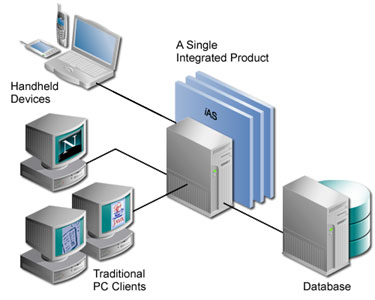
\includegraphics[width=0.7\textwidth]{images/vis.jpg}
	\caption{Tymczasowe zdjęcie architektury Klient-Serwer}
	\label{fig:KlientSerwer}
\end{figure}
\section{Java}
Java jest obiektowym wieloplatformowym językiem programowania. Jest ona jednym z najpopularniejszym języków dla deweloperów oprogramowania \cite{JavaMicrosoft}. Korzysta z wirtualnej maszyny Java (JVM), które mogą zostać zainstalowane na większości komputerów i urządzeń przenośnych. Został on stworzony z myślą ,,napisz raz, uruchamiaj w dowolnym miejscu''. 
\\W projekcie jest odpowiedzialny za logikę biznesową aplikacji, przetwarzanie danych oraz komunikację z bazą danych \cite{JDK21Docs}.
\subsection*{Spring Boot}
Framework Spring Boot pozwala znacząco uprościć proces tworzenia aplikacji webowej w Javie. Eliminuje konieczność ręcznej konfiguracji wielu elementów. Pełni on role fundamentu dla warstwy serwerowej, udostępniając interfejs REST API, który umożliwia komunikację przy użyciu odpowiednich punktów końcowych (ang. \textit{endpoints}). Składa się z takich rzeczy jak:
\begin{itemize}
	\item Controller - obsługuje żądania HTML
	\item Repository - odpowiada za komunikacje z bazą danych
	\item Config - Obejmuje konfiguracje aplikacji, polityki bezpieczeństwa, ciasteczka
	\item Model - Reprezentuje dane w postaci klas, które są odwzorowaniem tabel w bazie danych.
	\item Resource - Znajdują się w nim właściwości aplikacji, oraz statyczne elementy.
\end{itemize}
Spring Boot wspiera również takie mechanizmy jak Wstrzykiwanie zależności (ang. \textit{Dependency Injection}) oraz AOP (ang. \textit{Aspect-Oriented Programming}) \cite{SpringDocs}.
\subsection*{Maven}
W projekcie wykorzystano narzędzie Apache Maven, które pełni role automatyzacji budowy i zarządzania zależnościami. Pozwala zdefiniować wszystkie wymagane biblioteki i frameworki w jednym centralnym pliku pom.xml (ang. Project Object Model). Działa w oparciu o repozytoria, w których przechowywane są biblioteki. Główny plik zawiera takie informacje jak:
\begin{itemize}
	\item groupId, artifactId, version - identyfikatory projektu,
	\item sekcję dependencies - listę bibliotek, które mają zostać automatycznie pobrane,
	\item sekcję build - ustawienia dotyczące budowania aplikacji,
	\item sekcje plugins - narzędzia wspierające proces budowania
\end{itemize}
W przypadku aplikacji opartej na Spring Boot, Maven pobiera również tzw. startery np.:
\begin{itemize}
	\item spring-boot-starter-web - uruchamia aplikacje serwerową (np. Tomcat) i pozwala tworzyć kontrolery REST
	\item spring-boot-starter-data-mongodb - Umożliwia korzystanie z bazy mongo
	\item spring-boot-starter-security - Dodaje mechanizmy autoryzacji i uwierzytelniania
	\item spring-boot-starter-test - pozwala na testowanie aplikacji
\end{itemize}
Cała konfiguracja środowiska sprowadza się do utworzenia odpowiedniego pliku z zależnościami, a Spring Boot automatycznie na jego podstawie konfiguruje je przy uruchomieniu \cite{MavenDocs}.
\subsubsection*{Dane do wstawienia w ten rozdział}
 Korzysta między innymi z takich zależności jak: 
\begin{itemize}
	\item Lombok - Ułatwia tworzenie klas i podstawowych funkcji w klasach.
	\item DevTools - Pozwalające m.in. na przeładowanie w czasie rzeczywistym.
	\item Web - Zawiera RESTful API, pozwala na komunikacje.
	\item Security - Umożliwia zastosowanie zabezpieczeń i autoryzacji do kontrolowania aplikacji.
	\item MongoDB - Do przechowywania dokumentów w formacie zbliżonym do JSON.
	\item Validation - pozwala na walidacje pól na przykład: ustawienie długości pola, pole nie może być puste i tym podobne.
\end{itemize}
\section{React}
React to jedna z bibliotek JavaScript służąca do tworzenia interfejsów użytkownika (ang. User Interface) w aplikacjach webowych. Jest oparta na koncepcji komponentów, które można łatwo ze sobą łączyć i w czytelny sposób wyświetlać na stronie. React pozwala renderować widoki na podstawie mechanizmu Virtual DOM (ang. Document Object Model). Obiekt DOM umożliwia dostęp do struktury strony w celu jej modyfikacji. W przypadku modelu wirtualnego minimalizuje operacje na drzewie rzeczywistym. 
\subsection*{Vite}
W celu usprawnienia procesu tworzenia aplikacji zastosowano narzędzie Vite, które pełni rolę bundlera, czyli łączy ze sobą wiele plików m.in. kody źródłowe i zależności. Rozwiązanie to oferuje szybkie uruchamianie środowiska, optymalizacja kodu i co najważniejsze w usprawnieniu pracy poprzez przeładowanie kodu na bieżąco (ang. Hot Module Replacement), który pozwala wyświetlać zmiany bez konieczności ponownego budowania całej aplikacji. 
\subsection*{TypeScript}
Komponenty oraz wszystkie składowe projektu są przygotowane w języku TypeScript, który jest nadzbiorem języka JavaScript. Wprowadza on statyczne typowanie, znaczy to że typy są określone i sprawdzane w czasie kompilacji. Pozwala wprowadzać typy dla zmiennych, funkcji i obiektów. Dzięki temu kod jest bardziej czytelny i zrozumiały dla developera. 
\newline

Połączenie Reacta, Vite oraz TypeScript zapewnia wydajne i przyjemne środowisko dla pracy programisty, lepszą kontrole nad danymi i wydajność pracy. Technologie te zostały wybrane również dla bogatego wyboru bibliotek wspieranych przez react. Jedną z nich jest biblioteka AntD, która zawiera wstępnie przygotowane do użycia na stronie komponenty. 

\section{MongoDB}
MongoDB to nierelacyjna baza typu NoSQL. W przeciwieństwie do klasycznych baz relacyjnych MongoDB nie korzysta z tabel, lecz przechowuje dane w postaci dokumentów BSON (Binary JSON), które strukturą przypominają obiekty JSON.
Jeden dokument może mieć wiele różnych pól, co pozwala bardziej elastycznie modelować dane. Baza ta korzysta z kolekcji (ang. collections), które są odpowiednikami tabel w klasycznych bazach relacyjnych. Każdy wpis w bazie posiada własny unikatowy identyfikator \_id. Wspiera ona wiele operacji, takich jak sortowanie, filtrowanie, czy grupowanie. Zaimplementowanie ich w kodzie programu jest proste i wystarczy do tego odpowiednio utworzone repozytorium z odpowiednimi operacjami (lst. \ref{lst:java-repo}). Połączenie bazy w aplikacji Java odbywa się za pomocą modułu Spring Data MongoDB. To właśnie ten moduł odpowiada za możliwość tworzenia repozytorium.
\begin{lstlisting}[language={Java}, caption={Przykładowe repozytorium w Javie}, label={lst:java-repo}]
@RepositoryRestResource(collectionResourceRel = "users", path = "users")
public interface UserRepository extends MongoRepository<User, String> {
	Optional<User> findByLogin(String login);
	List<User> findByLoginContainingIgnoreCase(String loginPart);	
}	
\end{lstlisting}
Powyższy fragment kodu pozwala znaleźć użytkownika po loginie lub wyszukać wszystkich użytkowników zawierających podany ciąg znaków w swojej nazwie.
\begin{lstlisting}[caption={Przykladowy dokument z kolekcji}, label={lst:MongoDB-doc}]
{
	"id": "68d56ad95a544e07c8ebaa54",
	"login": "ADMIN",
	"password": "$2a$10$.itTB4jFiMBPdZSDebVE4Obtl8FpDiT7CHovqCtq8dcUnFMoe1gem",
	"role": "ADMIN"
}
\end{lstlisting}
